\chapter{Construção}
\label{chap:Construcao}

Para a construção do \emph{software} aplicativo, foi utilizado uma arquitetura em
três camadas: sensor, distribuidor de acesso (\emph{IoT gateway}) e apresentação
(\emph{Web}). Nesta divisão, os sensores capturam as informações dos dispositivos
e repassam para a camada seguinte, no \emph{gateway} todas as partes se
encontram para fornecer e solicitar informações e, por último, a camada de
apresentação coleta o que é enviado dos sensores e gera uma página \emph{Web}
para visualização dos dados capturados.

Esta divisão está de acordo com o padrão encontrado em outras aplicações
\emph{IoT} onde a última camada usualmente varia entre apresentação e mineração
de dados (\emph{Data Mining}).

A camada de sensor utilizou as tecnologias \emph{Node.js}, \emph{TShark} parte
do \emph{Wireshark} e \emph{MQTT.js}. A camada \emph{gateway} foi composta
basicamente pelo \emph{MQTT Broker} \emph{Mosquitto}. Por fim a camada de
apresentação utlizou as tecnologias \emph{Node.js}, \emph{MQTT.js}, \emph{html},
\emph{css}, \emph{javascript}, \emph{Bootstrap} e \emph{Google Maps API}.

\begin{figure}[htb]
	\caption{\label{fig-arq-app}Arquitetura da aplicação}
	\begin{center}
		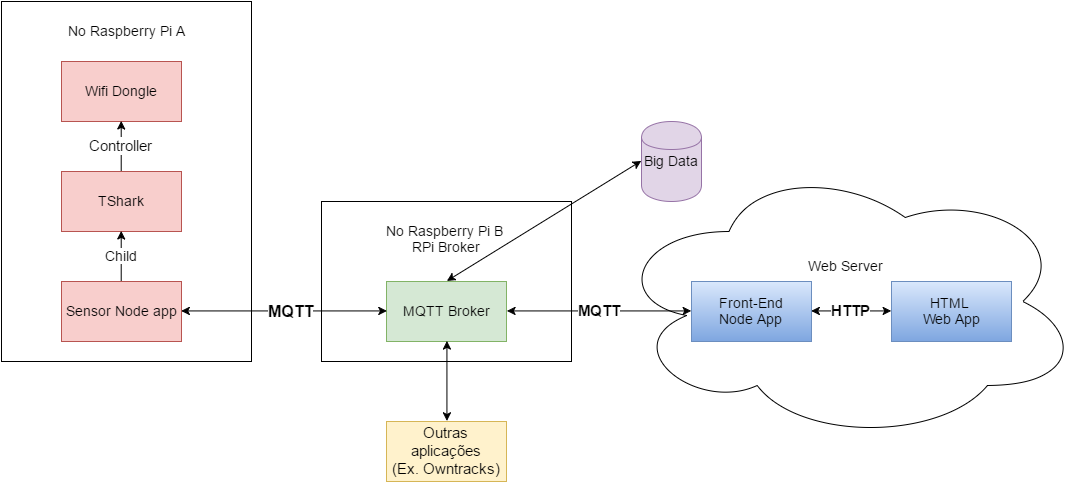
\includegraphics[width=1\textwidth]{050-construcao/esquema-proj.png}
	\end{center}
	\legend{Fonte: Elaborada pelo autor}
\end{figure}
